\documentclass[10pt,a4paper,titlepage,oneside]{article}
\usepackage{LabProtocol}

\exercise{Exercise I}

% enter your data here
\authors{

	Mihai-Andrei Dancu, Matr. Nr. 12123694 \par
	{\small e12123694@student.tuwien.ac.at} \par
}


\begin{document}

\maketitle


%████████╗ █████╗ ███████╗██╗  ██╗     ██╗
%╚══██╔══╝██╔══██╗██╔════╝██║ ██╔╝    ███║
%   ██║   ███████║███████╗█████╔╝     ╚██║
%   ██║   ██╔══██║╚════██║██╔═██╗      ██║
%   ██║   ██║  ██║███████║██║  ██╗     ██║
%   ╚═╝   ╚═╝  ╚═╝╚══════╝╚═╝  ╚═╝     ╚═╝
\Task{Introduction and Preparations}


\begin{qa}{After adding the PLL, the connections of the two clocks to the rest of the system as a whole can be seen in \textbf{Figure 1}.}
	\begin{center}
		\begin{figure}[h!]
			\centering
				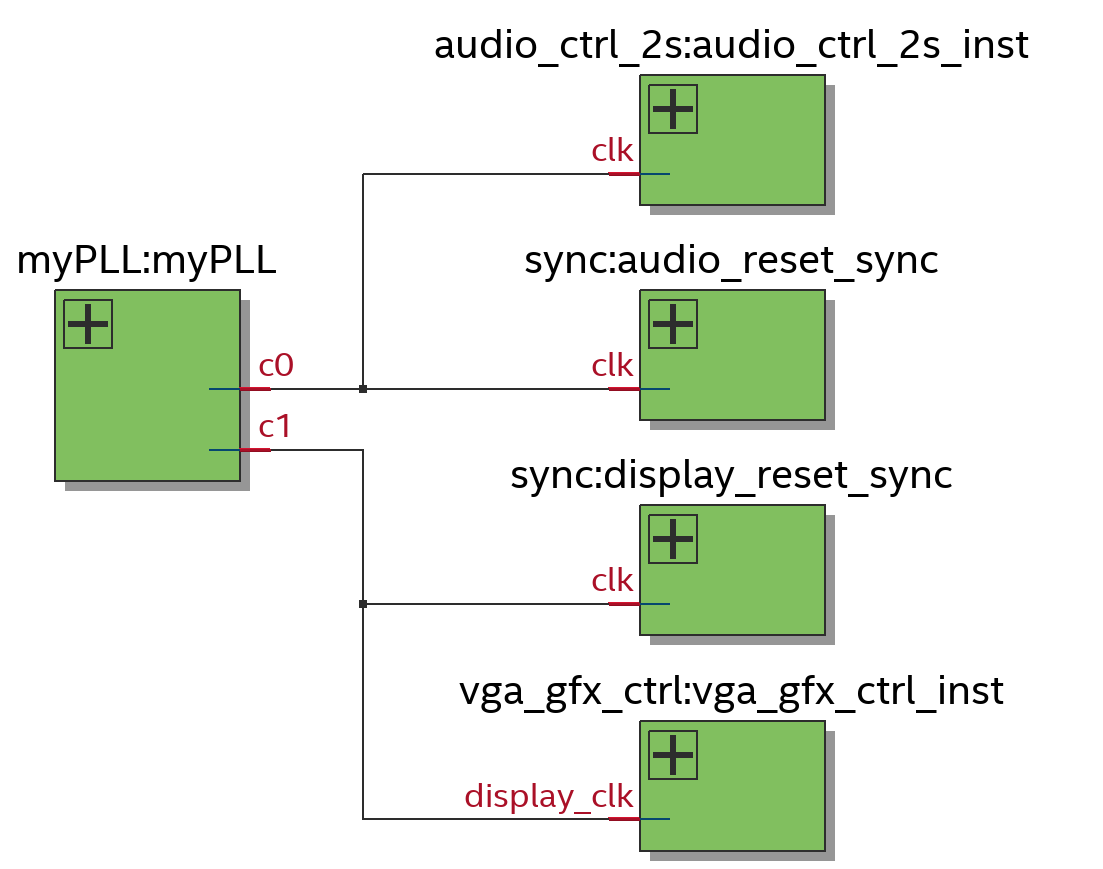
\includegraphics[width=0.5\linewidth]{pll.png}
			\caption{RTL netlist viewer screenshot filtered}
		\end{figure}
	\end{center}
\end{qa}
%%%%%%%%%%%%%%%%%%%%%%%%%%%%%%%%%%%%%%%%%%%%%%%%%%%%%%%%%%%%%%%%%%%%%%%%%%%%%%%%


%████████╗ █████╗ ███████╗██╗  ██╗    ██████╗ 
%╚══██╔══╝██╔══██╗██╔════╝██║ ██╔╝    ╚════██╗
%   ██║   ███████║███████╗█████╔╝      █████╔╝
%   ██║   ██╔══██║╚════██║██╔═██╗     ██╔═══╝ 
%   ██║   ██║  ██║███████║██║  ██╗    ███████╗
%   ╚═╝   ╚═╝  ╚═╝╚══════╝╚═╝  ╚═╝    ╚══════╝
\Task{Seven-Segment Display Controller}


\begin{qa}{ After designing and implementing the FSM, a ressource usage analysis has been conducted which provided the following results:}

\centering
\begin{tabular}{l|ll}
	\hline
		                   & Combinational ALUTs & Dedicated Logic Registers  \\ \hline\hline 
	Absolute number            & 508                 & 196                        \\
	\% of whole design         & 7.21                & 4.74                       \\
	\% of whole FPGA resources & 0.44                & 0.17                       \\ \hline
\end{tabular}
\end{qa}

\newpage

\begin{qa}{The state graph of the state machine can be seen in \textbf{Figure 2}. In \textbf{IDLE} mode, the SSDs display the displacement of the two controller
	   sticks in form of hexadecimal numbers. By pressing the switch the state machine switches into \textbf{CONVERT} mode, where the output number is computed, then automatically
	   switches to \textbf{DISPLAY} mode where the displacement of the chosen stick on the chosen axis is displayed in decimal form. Furthermore, should the sign switch be pressed, 
           the number switches between signed and unsigned representation. Should any of the parameters change (i.e., the controller input, the chosen stick or axis or the sign
           switch), the \textbf{CONVERT} mode is entered again to update the result which is then again displayed in \textbf{DISPLAY} mode. Once in \textbf{DISPLAY}, one can
	   switch back to \textbf{IDLE} mode anytime by pressing the switch. Furthermore, no changes may be made to the input parameters while in \textbf{CONVERT} mode and the ouput while
	   in this mode is blank.}

\begin{figure}[h!]
	\centering
	\includegraphics[width=0.75\linewidth]{dia/pdf/fsm.pdf}
\end{figure}

\end{qa}

%%%%%%%%%%%%%%%%%%%%%%%%%%%%%%%%%%%%%%%%%%%%%%%%%%%%%%%%%%%%%%%%%%%%%%%%%%%%%%%%

%████████╗ █████╗ ███████╗██╗  ██╗    ██████╗ 
%╚══██╔══╝██╔══██╗██╔════╝██║ ██╔╝    ╚════██╗
%   ██║   ███████║███████╗█████╔╝      █████╔╝
%   ██║   ██╔══██║╚════██║██╔═██╗      ╚═══██╗
%   ██║   ██║  ██║███████║██║  ██╗    ██████╔╝
%   ╚═╝   ╚═╝  ╚═╝╚══════╝╚═╝  ╚═╝    ╚═════╝ 
\Task{Decimal Printer}

\begin{qa}{Include the image or images produced by your graphics command interpreter testbench (not the game testbench).}


\begin{figure}[h!]
	\centering
	% \includegraphics[width=1.0\linewidth]{your filename here}
	\dummyimage
	\caption{Testbench output}
\end{figure}

\end{qa}

\end{document}
